% Section content template for individual Educative lessons
% This file contains the actual content for a specific section
% Generated from Educative API section content

% Section: AWS Kinesis Outage Affecting Many Organizations
% Section ID: 5243362298298368
% Section Slug: aws-kinesis-outage-affecting-many-organizations
% Generated: 2025-12-08T15:37:39.597710

\textbf{Amazon Kinesis} allows us to aggregate, process, and analyze real-time streaming data to get timely insights and react quickly to the information it provides. It continuously captures gigabytes of data from hundreds of thousands of sources per second. The Kinesis service's frontend handles authentication, throttling, and distributes workloads to its back-end ``workhorse'' cluster via database sharding. On November 25, 2020, the Amazon Kinesis service was disrupted in the US-East-1 (Northern Virginia) region, affecting thousands of other third-party services. The failure was significant enough to take out a large portion of Internet services.

\begin{figure}[htbp]
 \centering
 
\includegraphics[width=0.15\textwidth]{Images/chapter_42/section_5243362298298368/4919051352801280.png}
 
\end{figure}

\subsection{Sequence of events}\label{A1nPITaifE1FrevqG98fK}

\begin{itemize}
\item
\protect\phantomsection\label{vfQi54OtqjjFj4qSPd97f}
According to Amazon, the event was triggered by adding a small capacity to the AWS front-end fleet of servers, scheduled from 2:44 a.m. PST to 3:47 a.m. PST.
\item
\protect\phantomsection\label{-Kvj0IQHrZ1rx-Xrbz00p}
The addition of the new capacity caused all the servers in the fleet to exceed the maximum number of threads that are allowed by an operating system configuration.
\item
\protect\phantomsection\label{WySWrwaFL6LwIJEiT1CGa}
Due to exceeding the limit on threads, cache construction was failing to complete, and front-end servers were ending with useless shard maps that left them unable to route requests to back-end clusters.
\item
\protect\phantomsection\label{kFw1vi-NcNesdarcYVqsK}
Other primary Amazon services also stopped working, including Amazon Cognito and CloudWatch.

\begin{itemize}
\item
Kinesis Data Streams is used by Amazon Cognito to gather and analyze API usage patterns. Because of the long-running issue with Kinesis Data Streams, a hidden error in the buffering code---which is required for Cognito services---caused the Cognito web servers to start blocking on the backlogged Kinesis Data Stream buffers. As a result, Cognito customers witnessed an increase in API failures and latencies for Cognito user pools and identity pools, making it impossible for external users to authenticate or receive temporary AWS credentials.
\item
CloudWatch uses Kinesis Data Streams to process metrics and log data. The
\texttt{PutMetricData} and \texttt{PutLogEvents} APIs in CloudWatch encountered higher error rates and latencies, and alerts were set to INSUFFICIENT\ DATA. The great majority of metrics were unable to be processed due to higher error rates and latencies. When
CloudWatch was experiencing these greater issues, internal and external clients couldn't persist all metric data to the CloudWatch service.
\end{itemize}
\end{itemize}

\begin{figure}[htbp]
 \centering
 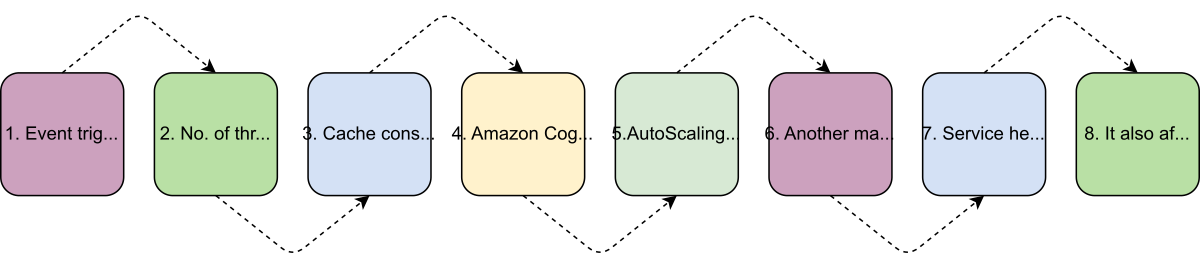
\includegraphics[width=0.5\textwidth]{Images/chapter_42/section_5243362298298368/4981033166700544.png}
 \caption{Sequence of events }
\end{figure}

\begin{itemize}
\item
\protect\phantomsection\label{fGqB2GXb4bJiSmeFB5AMT}
Due to the problems with CloudWatch metrics, two services were also impacted. First , AutoScaling policies that rely on CloudWatch measurements suffered delays. Second, Lambda experienced the effect. Currently
, posting metric data to CloudWatch is required as a part of the Lambda function invocation. If CloudWatch is unavailable, Lambda metric agents are meant to buffer metric data locally for a period of time. The metric data buffering became so large that it generated memory congestion on the underlying service hosts utilized for Lambda function invocations, leading to higher error rates.
\item
\protect\phantomsection\label{Bxfe_yPv2Cc5ueRvn1cDH}
Increased API failures and event processing delays plagued CloudWatch Events and EventBridge. Event Bridge is used by Elastic Container Service (ECS) and Elastic Kubernetes Service (EKS) to drive internal processes for managing client clusters and jobs. This has an impact on new cluster provisioning, existing cluster scaling, and task deprovisioning.\hspace{0pt}\hspace{0pt}
\item
\protect\phantomsection\label{OKIciaQKBLoZuQMszXGBC}
Apart from the service issues, Amazon also experienced delays in communicating service status to their customers. Amazon uses two dashboards for communication with their customers, Service Health Dashboard and Personal Health Dashboard. The Service Health Dashboard informs all customers of events, such as the current one. It was down because of its dependency on Cognito, which was impacted by this event.
\item
\protect\phantomsection\label{xffBmzsACWZ5En-GByMjl}
Apart from the disruption in the Amazon services, this also had a ripple effect on thousands of third-party online services, applications, and websites. This includes Adobe Spark, Acorns, Coinbase, \emph{Washington Post}, and hundreds of such services.
\end{itemize}

\subsection{Analysis}\label{INfZ0bJNySQ1AjgWyfsvA}

\begin{itemize}
\item
\protect\phantomsection\label{Gp35N3zqd-9ltfJH1XJSO}
\textbf{Complexity of enhancing scalability}: We've been stressing the need for horizontal scalability in all of our design problems. This outage event shows that in practice, adding more capacity to a serving cluster so that we don't deny any client requests can be challenging and can have unintended side effects.
\item
\protect\phantomsection\label{NSJBWNHXui8HOpoApgaXv}
\textbf{The need for a trained team}: Training the production team to deal with such unforeseen situations is a challenging task, but it's worth it and can result in expedited recovery. In addition, randomly restarting the front-end servers and suspecting that the memory pressure causes the problem alludes to the challenges of reaching the root causes under the stress of time.
\item
\protect\phantomsection\label{YPfb5z1eO7Su_eM8NZR13}
\textbf{Reading from authoritative servers during bootstrap}: During the bootstrap process, it's a good idea to take data from the authoritative metadata store rather than from the front-end servers to reduce the impact of such failures.
\item
\protect\phantomsection\label{fU9kB1wSumZIK_uhwdUYo}
\textbf{Identification of faults in initial stages}: There's a need for automated processes to identify the causes of failure within the initial stages of its occurrence.
\item
\protect\phantomsection\label{5M3zdZBXRC6g7nIZPNjCP}
\textbf{Proper testing mechanisms can reduce the severity of the fault}: The new capacity that's causing the servers in the fleet to exceed the maximum number of threads is a potential bug that should have been fixed earlier than before restarting the servers. This reflects the inability to properly test the system. There should be a kind of simulator to test all cases before deploying additional capacity into the fleet.
\end{itemize}

\begin{figure}[htbp]
 \centering
 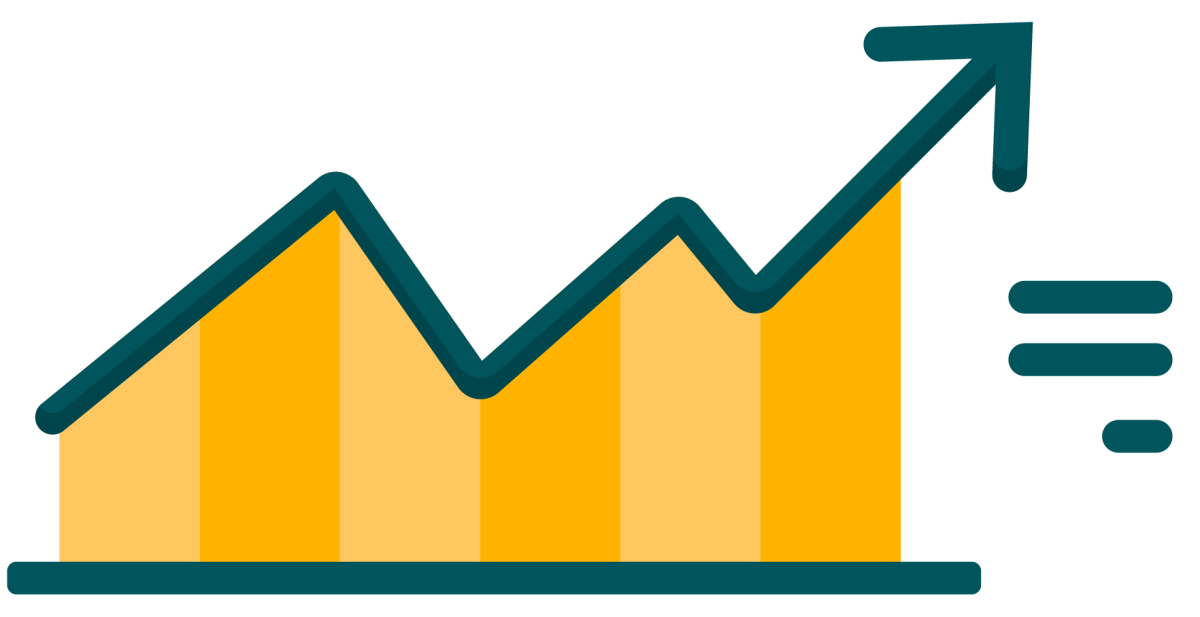
\includegraphics[width=0.15\textwidth]{Images/chapter_42/section_5243362298298368/5724714547019776.png}
 
\end{figure}

\begin{itemize}
\item
\protect\phantomsection\label{elWcRlZbwhZATD0vUMW0y}
\textbf{Finding potential bugs before planned events}: The issue with Kinesis Data Streams triggered a latent bug in the buffering code that caused the Cognito web servers to begin to block on the backlogged Kinesis Data Stream buffers. The potential bugs should be identified and fixed before critical planned events, such as adding capacity or software and hardware maintenance.
\item
\protect\phantomsection\label{Vw_JOA1pUph9Ayrs96DHA}
\textbf{Adopting automated processes for resource allocation}: The Cognito team sought to reduce~the effect of the Kinesis faults in the early phases of the event by providing extra capacity and therefore boosting their ability to buffer calls to Kinesis. Instead of manually assigning capacity, there should be an automated system to increase or reallocate capacity in such events.
\end{itemize}

\subsection{Lessons learned}\label{TFhUcq8uZreb_XE6ROX2X}

\begin{itemize}
\item
\protect\phantomsection\label{mQj_75aNFK4Sgq-dQi_5f}
\textbf{Testing}: Proper testing and identifying the potential bugs are essential. In this case, the number of threads exceeding a maximum limit defined by the operating system seems to be a possible bug.
\item
\protect\phantomsection\label{WUBIGuHPIqWJM8ksqmmjP}
\textbf{Ready operations team}: A bug bringing an overall system to a halt is the single point of failure, which is possible in a complex system. The production team should be trained and ready for such events.
\item
\protect\phantomsection\label{GeV8HDT5DQFJ-GiiPlss0}
\textbf{Reducing the number of servers}: To get significant headroom in the thread count used as the total threads, there's a need to move to more powerful CPU and memory servers. This will reduce the total number of servers and the threads required by each server to communicate across the fleet. Having fewer servers means that each server maintains fewer threads. Amazon is adding fine-grained alarming for thread consumption in the service.
\item
\protect\phantomsection\label{xAZHcksg4S6-wkipQR0M0}
\textbf{Front-end fleet changes}: Several changes are required to radically improve the cold start time for the front-end fleet. Moreover, the front-end server cache needs to be moved to a dedicated fleet.
\item
\protect\phantomsection\label{AS4y1GdoZG5St3obTpTG-}
\textbf{Avoiding recurrent failures}: To avoid recurrent failures in the future, extensive AWS services, like CloudWatch and others, must be moved to a separate, partitioned front-end fleet.
\end{itemize}

\begin{figure}[htbp]
 \centering
 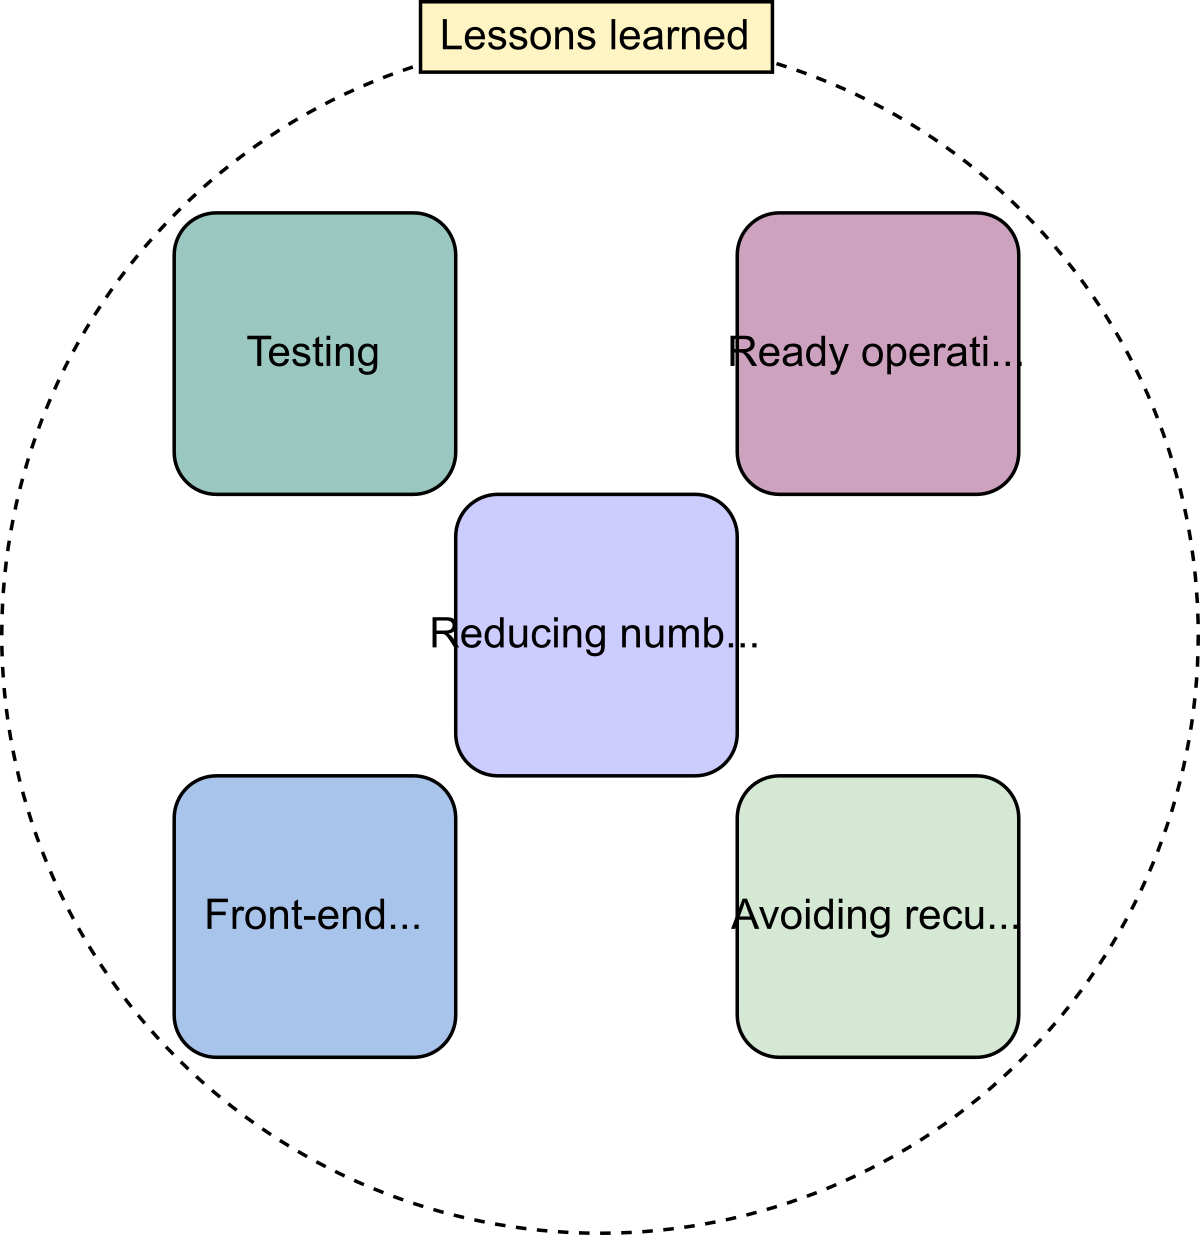
\includegraphics[width=0.25\textwidth]{Images/chapter_42/section_5243362298298368/6288810375905280.png}
 \caption{Lessons learned during the Kinesis outage}
\end{figure}

\begin{quote}
\textbf{Quiz:}
\textbf{Question 1:} What possible measures should Amazon have adopted to safeguard against the kind of failures they faced in Kinesis Data Streams?
\textbf{Answer:}  Possible solutions Dividing the region into independent failure domains would have reduced the blast radius of the event and made it possible for the production team to quickly recover from the problem.

They should have a system like Facebook\textquotesingle s Resource Allowance System for capacity reservation at the time of planned and unplanned events. Building an application across multiple clouds or
AWS regions would have made it easier for the affected customers to recover quickly. There\textquotesingle s a need to uncouple services to an extreme extent to eliminate cross-dependency issues. Failures in a complex system are inevitable. However, some important services like the status dashboard should be hosted on different servers, either inside the service or in some third-party's infrastructure.
\end{quote}



% End of section content